\documentclass[14pt]{beamer}
\setbeamertemplate{navigation symbols}{}
\usepackage{beamerthemesplit}

%\usepackage{fontspec}
%\setmainfont{Lucida Grande}
%\setmonofont{Monaco}

\setbeamertemplate{enumerate item}{%
    \usebeamercolor[bg]{item projected}%
    \raisebox{1.6pt}{\colorbox{bg}{\color{fg}\footnotesize\insertenumlabel}}%
}

\newcommand\FontSrc{\fontsize{6}{5}\selectfont}

%\beamertemplatenavigationsymbolsempty
%\setbeamerfont{page number in head/foot}{size=\small}
%\setbeamertemplate{footline}[frame number]

\usepackage{listings}
\lstset{
    language=C++,
    breakatwhitespace,
    columns=fullflexible,
    keepspaces,
    breaklines,
    tabsize=4, 
    basicstyle=\ttfamily,
    keywordstyle=\color{blue},
    stringstyle=\color{red}\ttfamily,
    commentstyle=\color{green}\ttfamily,
    showstringspaces=false,
    extendedchars=true,
}

\begin{document}

\defverbatim[colored]\lstfnw{
    \begin{lstlisting}[tabsize=4,basicstyle=\footnotesize\ttfamily]
auto fnw = [&probs](int k, int p1, int p2) -> double {
    const double parm = 0.000001f;
    const double d = std::fabs(probs[p1][k] - probs[p2][k]);
    const double w = 1.f / (1 + d / parm);
    return w;
};  
\end{lstlisting}
}

\defverbatim[colored]\lstfnlij{
    \begin{lstlisting}[tabsize=4,basicstyle=\footnotesize\ttfamily]
auto fnlij = [fnadj, fnisadj, fnw](int k, int p1, int p2, double& v) -> bool {
    v = 0;
    if (p1 == p2) {
        auto adj = fnadj(p1);
        for (int p: adj) {
            v += fnw(k, p1, p); 
        }   
    } else if (fnisadj(p1, p2)){
        v = -fnw(k, p1, p2);
    } else {
        return false;
    }   
    return true;
};
\end{lstlisting}
}

\defverbatim[colored]\lstmtx{
    \begin{lstlisting}[tabsize=4,basicstyle=\footnotesize\ttfamily]
    SparseMatrix<double, ColMajor> lu(usize, usize);
    MatrixRd bt(usize, msize);
    MatrixRd xm(msize, 1); 
    ................
    ................
    const auto& rightside = bt * xm;
    SparseLU<SparseMatrix<double, ColMajor>> solver(lu);
    const auto& pk = solver.solve(rightside);
    ................
    ................
\end{lstlisting}
}

\title{Image Graph For Semi-Automatic Segmentation}  
\author{Yanhui Shen @ zjnu}

\begin{frame}
    \date{\today} 
    \titlepage
\end{frame}

\begin{frame}{Contents}
    \begin{enumerate}
        \item Semi-Automatic Segmentation
        \item Random Walks Algorithm
        \item Calculation of Edge Weights
        \item Implementation
        \item Experiment Result
    \end{enumerate}
\end{frame}

\begin{frame}{Semi-Automatic Segmentation}
    Also known as interactive image segmentation.
    \newline\newline
    Given a small number of pixels with user-defined labels,
    let the algorithm learn a pattern from them.
    \newline\newline
    Then the algorithm will decide the rest pixels belong to which label,
    thus a image segmentation can be obtained.
\end{frame}

\begin{frame}{Random Walks Algorithm}
    \begin{columns}
        \column{0.4\textwidth}
        Assume that we have a graph with three nodes labeled.
        \newline\newline
        What will the color be for the rest of unlabed nodes?
        \column{0.6\textwidth}
        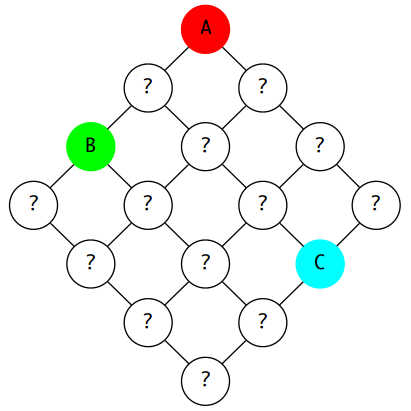
\includegraphics[scale=0.45]{eg1.png}
    \end{columns}
\end{frame}
\begin{frame}{Random Walks Algorithm}
    \structure{Dirichlet integral:}
    \[
        D[u] = \frac{1}{2} \int_{\Omega} \mid \nabla u\mid ^2 d\Omega
    \]
\end{frame}
\begin{frame}{Random Walks Algorithm}
    \structure{Discrete calculus:}
    \begin{equation*}
        \begin{split}
            D[x] &= \frac{1}{2} x^TLx \\
                 &= \frac{1}{2} 
            \left[
                \begin{array}{cc}
                    x_m^T & x_u^T
                \end{array}
            \right]
            \left[
                \begin{array}{cc}
                    L_m & B \\
                    B^T & L_u
                \end{array}
            \right]
            \left[
                \begin{array}{cc}
                    x_m \\
                    x_u
                \end{array}
            \right] \\
            &= \frac{1}{2}(x_m^T L_m x_m + 2 x_u^T B^T x_m + x_u^T L_u x_u)
        \end{split}
    \end{equation*}
\end{frame}
\begin{frame}{Random Walks Algorithm}
    \structure{Differentiating $D[x_u]$ with respect to $x_u$:}
    \begin{equation*}
        \begin{split}
            D[x_u] &= \frac{1}{2}(x_m^T L_m x_m + 2 x_u^T B^T x_m + x_u^T L_u x_u) \\
            \frac {\partial D[x_u]} {\partial x_u} &= B^Tx_m + L_u x_u
        \end{split}
    \end{equation*}
    \pause
    \structure{Critical point yields:}
    \[
        let \quad \frac {\partial D[x_u]} {\partial x_u} = 0
        \quad \Rightarrow \quad
        \setlength{\fboxrule}{2pt}
        \fcolorbox{red}{white}{$L_u x_u = - B^T x_m$}
    \]
\end{frame}
\begin{frame}{Random Walks Algorithm}
    \structure{$L^k$ satisfying:}
    \[
        L_{ij}^k = 
        \begin{cases} 
            \delta_i^k ,\quad & if\ i=j \\
            -w^k(v_i, v_j) ,\quad & if\ i\ and\ j\ are\ adjacent \\
            0, \quad & otherwise
        \end{cases}
    \]
    \pause
    \structure{Degree of a vertex $v_i$ is:}
    $\delta_i^k = \sum_{j \in adj(j)} w^k(v_i, v_j)$
\end{frame}

\begin{frame}{Calculation of Edge Weights}
    \structure{Color space:}
    \begin{columns}
        \column{0.5\textwidth}
        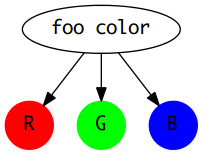
\includegraphics[scale=0.45]{rgb.png} \pause
        \column{0.5\textwidth}
        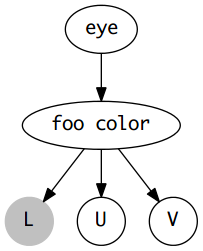
\includegraphics[scale=0.45]{luv.png}
    \end{columns}
\end{frame}
\begin{frame}{Calculation of Edge Weights}
    \structure{Nonparametric density estimation:}
    \begin{columns}
        \column{0.5\textwidth}
        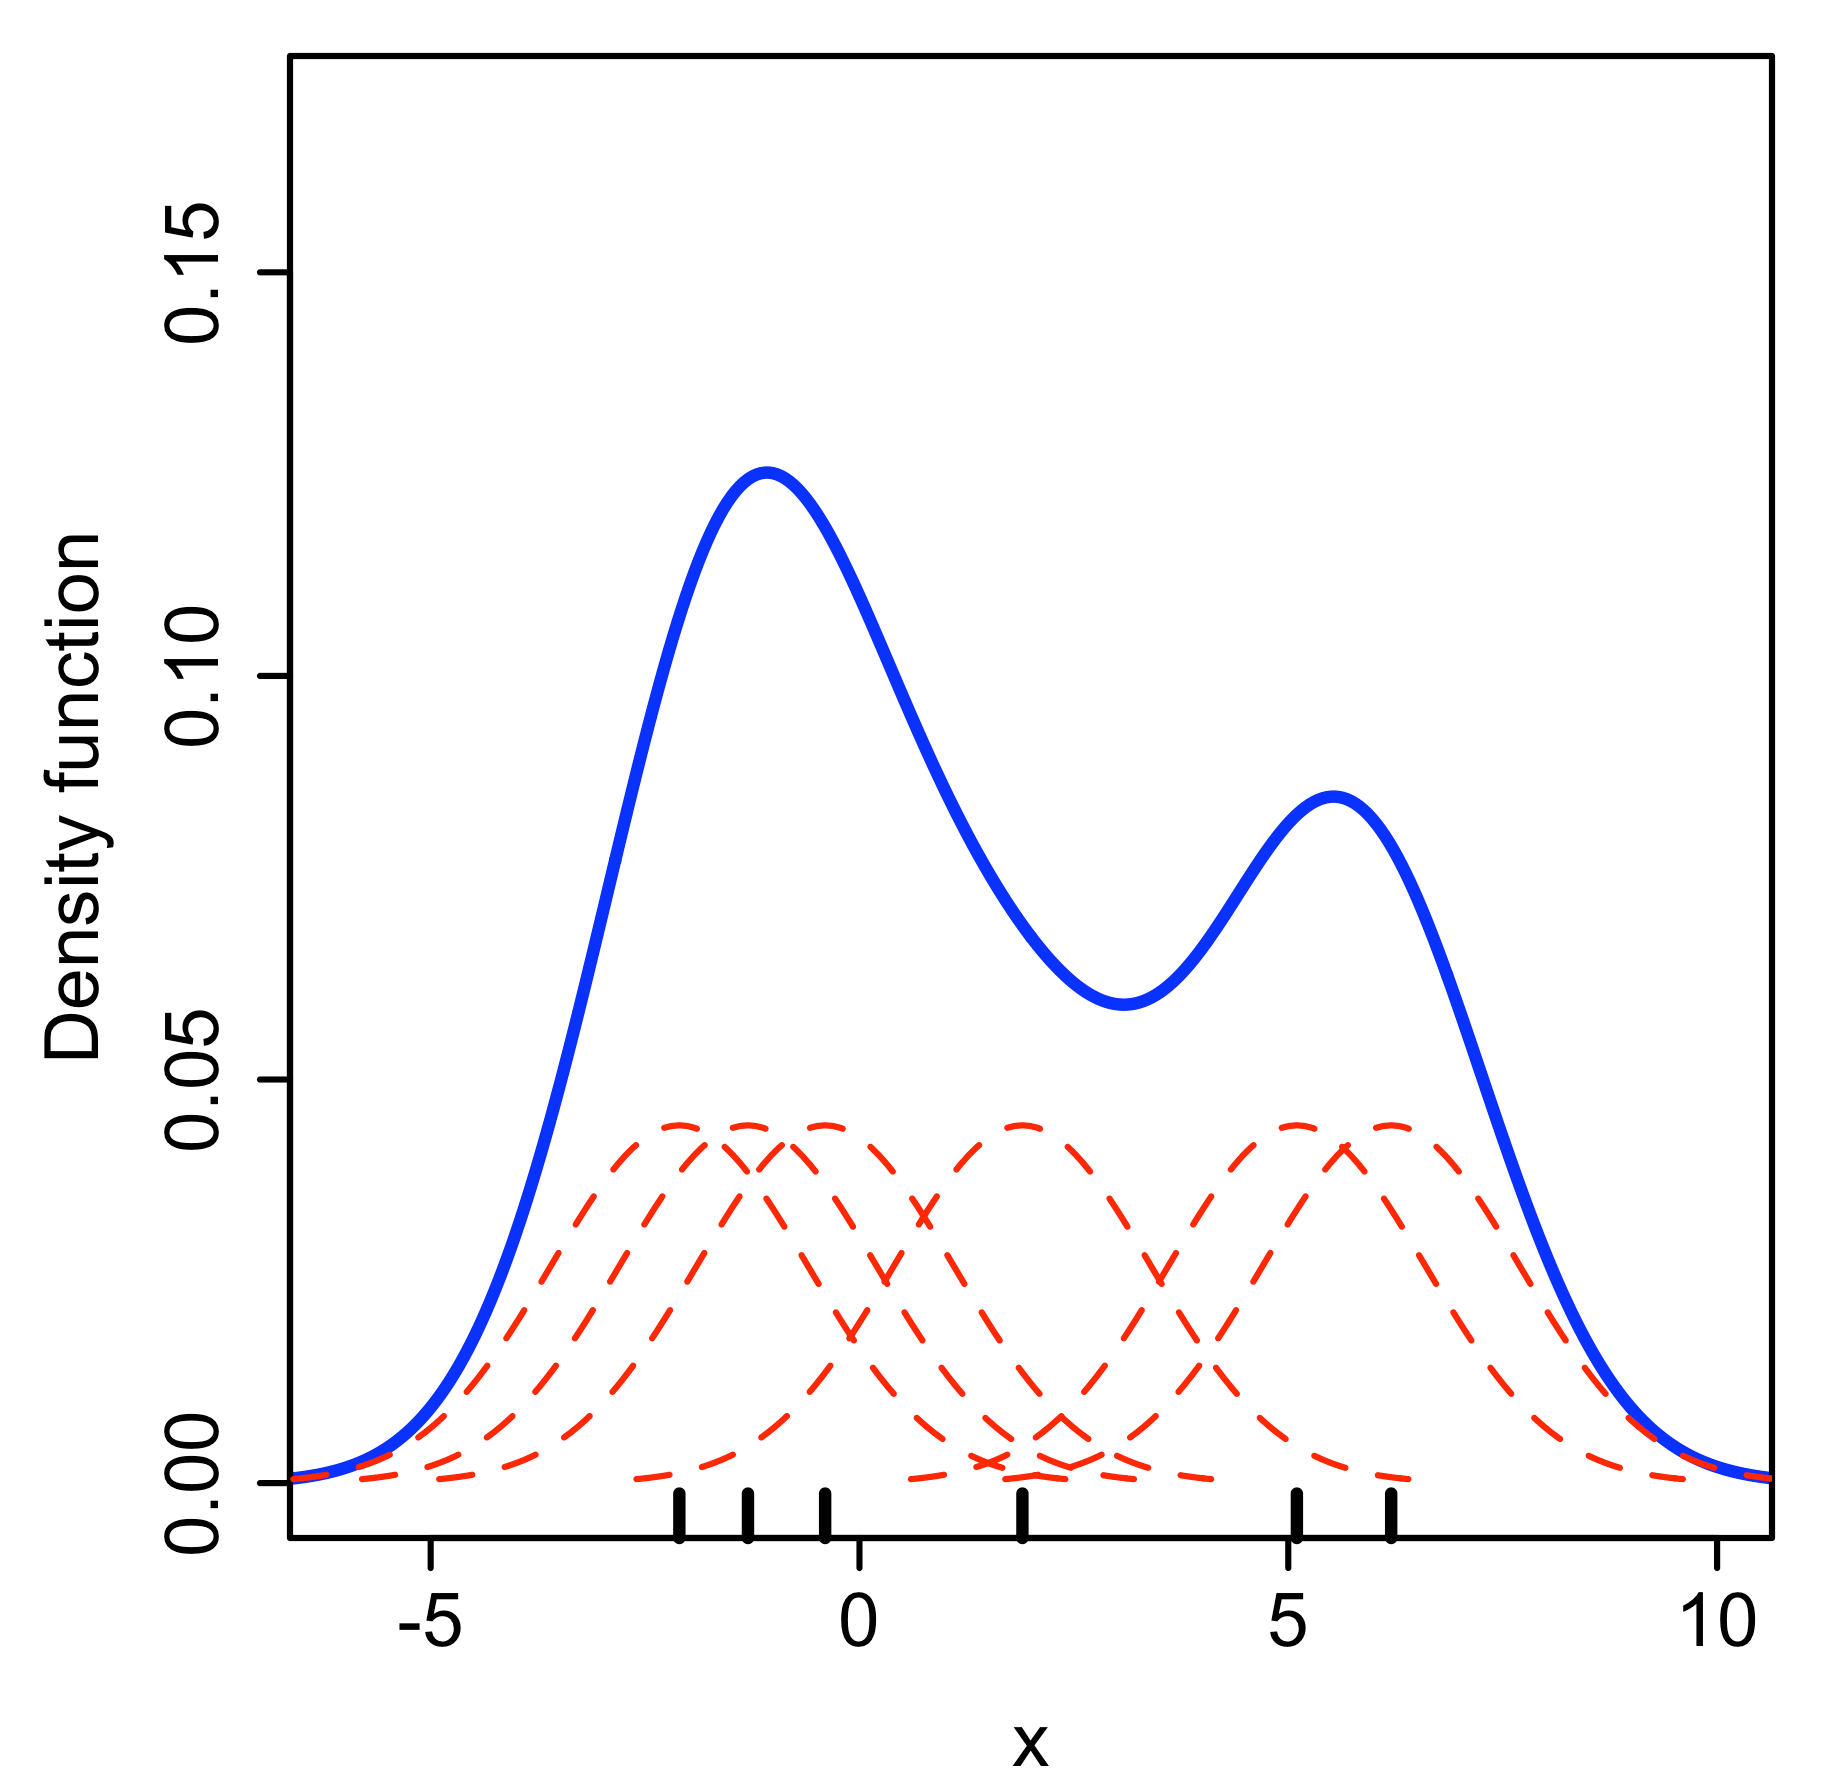
\includegraphics[scale=0.08]{kde.png} \pause
        \column{0.5\textwidth}
        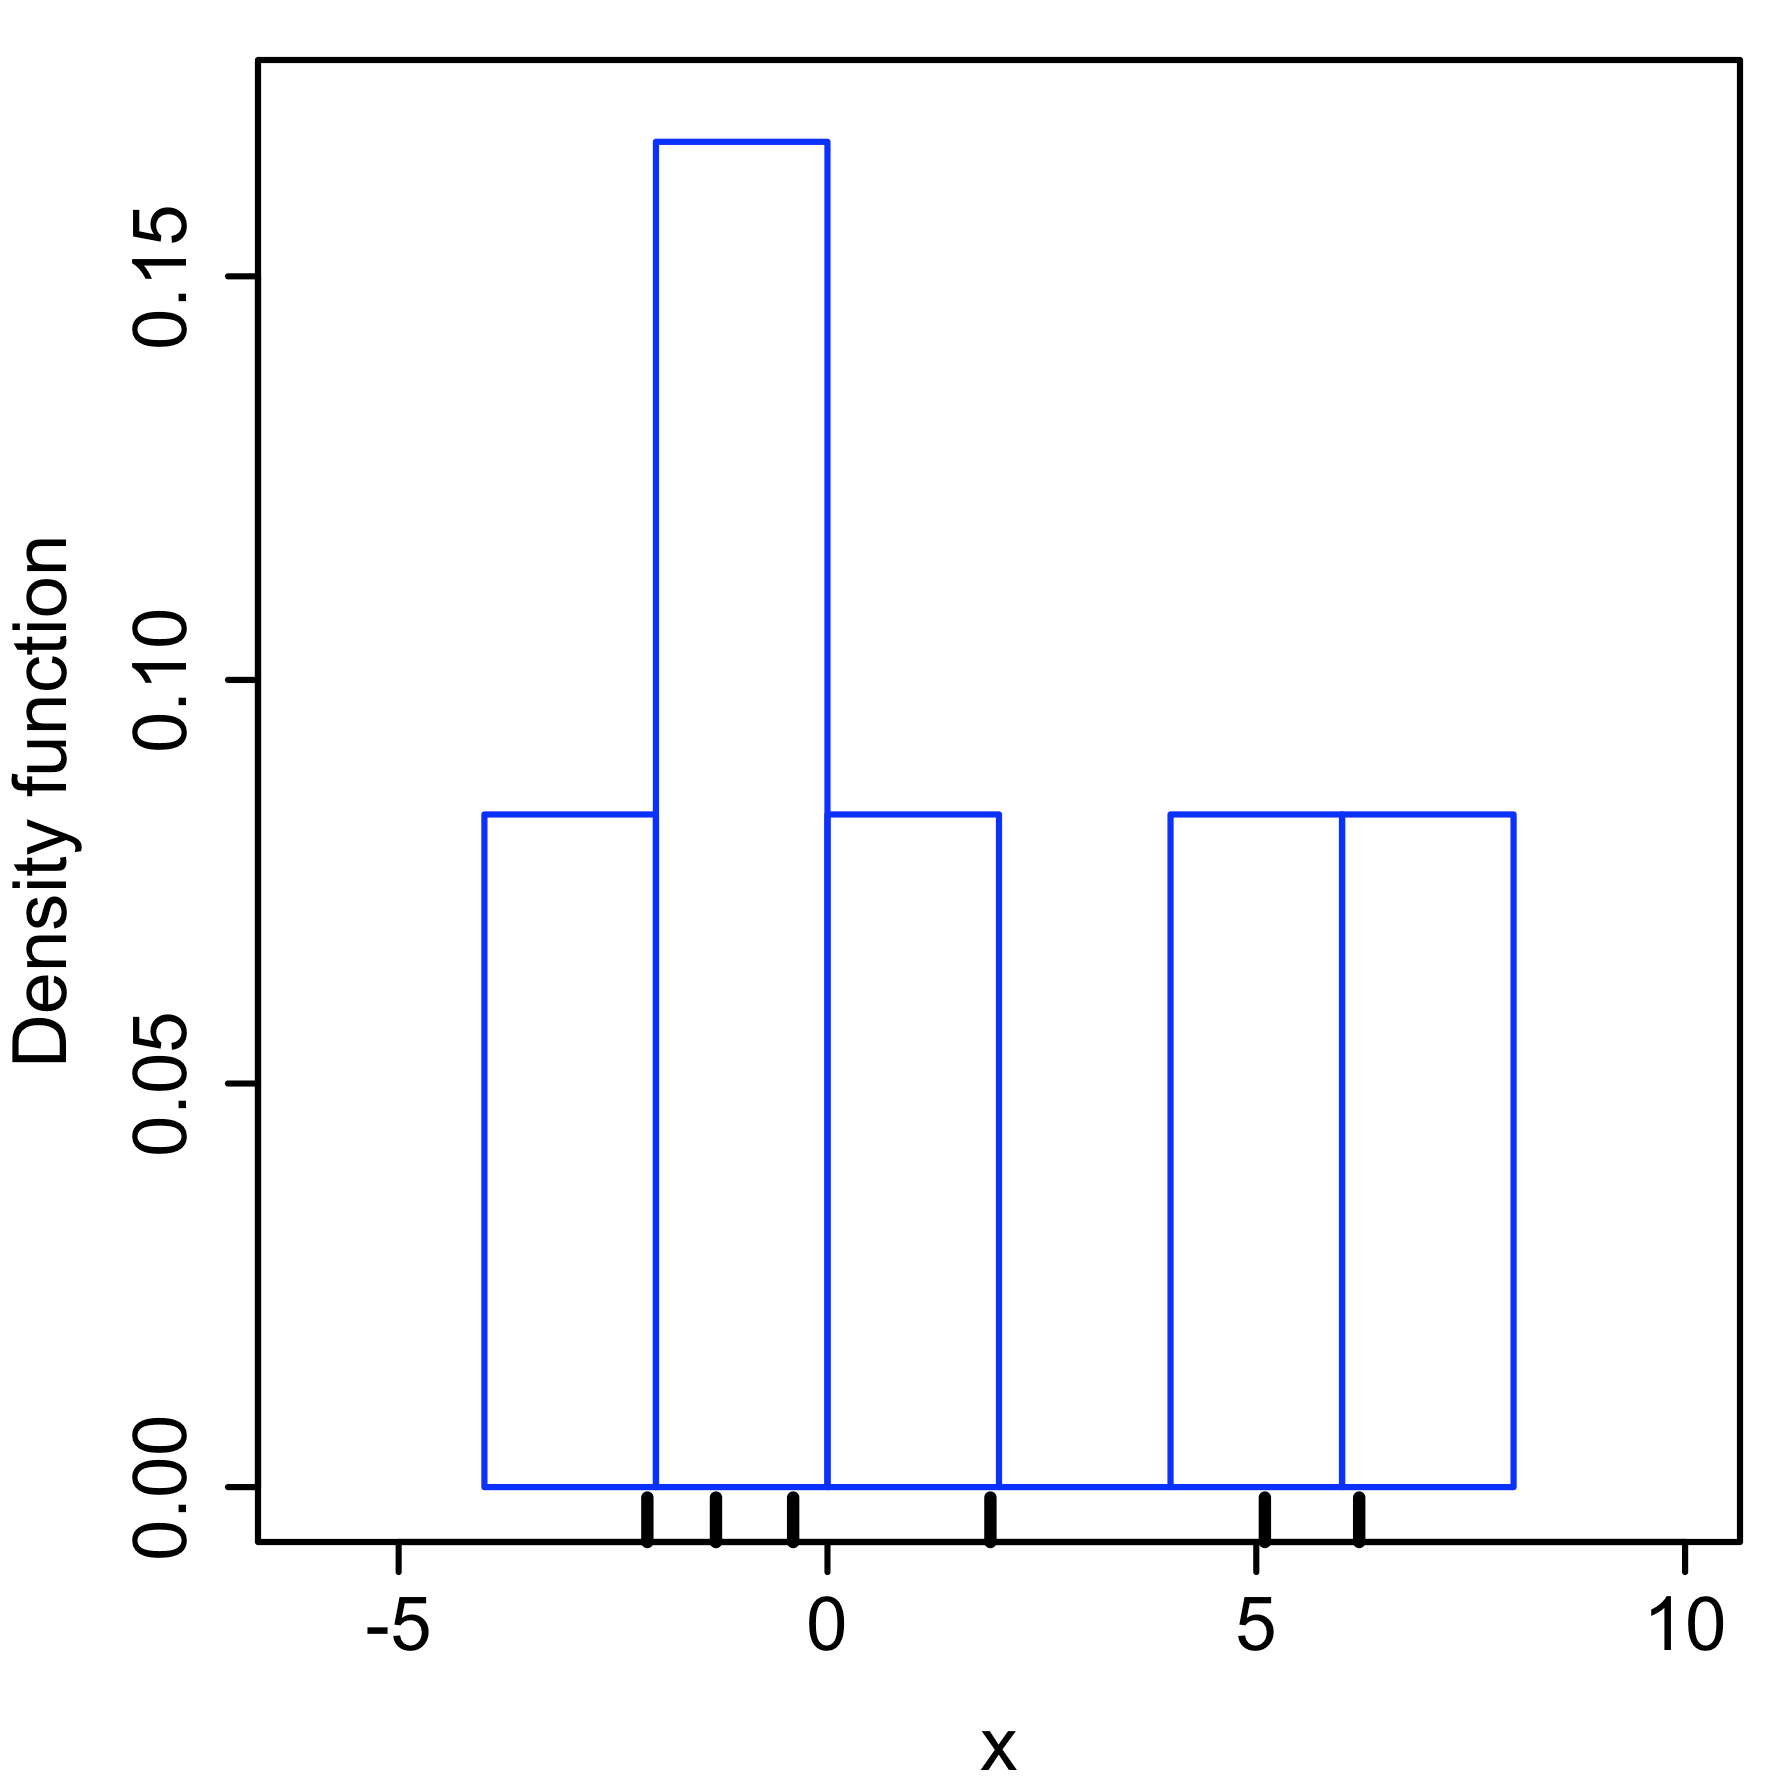
\includegraphics[scale=0.08]{histogram.png}
    \end{columns}
\end{frame}
\begin{frame}{Calculation of Edge Weights}
    \structure{Calculate degree with following equations:}
    \[
        \begin{cases}
        \pi_i^k = prob(v_i \in obj_k \mid z(v_i)=z) \\
        d^k(v_{i}, v_{j}) = \mid \pi_i^k - \pi_j^k \mid \\
        w^{k}(v_{i}, v_{j}) = \frac{1}{1+d^{k}(v_{i}, v_{j})/\sigma}
    \end{cases}
    \]
\end{frame}

\begin{frame}{Implementation}
    \structure{Tools:}
    \begin{itemize}
        \item C++11, Clang Compiler
        \item Eigen for matrix math
        \item Qt toolkit
    \end{itemize}
\end{frame}
\begin{frame}{Implementation}
    \structure{Segmentation Scheme:}
    \begin{itemize}
        \item Learn Densities
        \item Conditional Probablities
        \item Edge Weights
        \item Laplcians
        \item Random Walker Probabilities
        \item Segmentation
    \end{itemize}
\end{frame}
\begin{frame}{Implementation}
    \structure{Edge weight:}
    \lstfnw
\end{frame}
\begin{frame}{Implementation}
    \structure{Laplacian Matrix:}
    \lstfnlij
\end{frame}
\begin{frame}{Implementation}
    \structure{Solve K linear systems:}
    \lstmtx
\end{frame}

\begin{frame}{Experiment Result}
    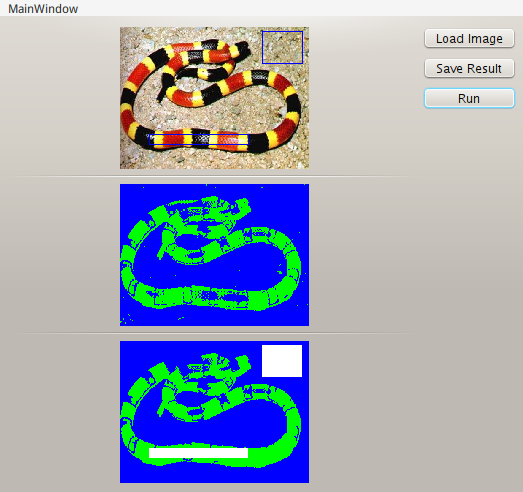
\includegraphics[scale=0.45]{snake1.png}
\end{frame}

\begin{frame}{EOF}
    Thank You!
\end{frame}

\end{document}
